% Copy Pasted any package used in ref so things work without me thinking about it
\documentclass{beamer} %best tool ever 100% worth it
\usepackage[utf8]{inputenc}
\usepackage{tikz}
\usetikzlibrary{automata, positioning, arrows.meta}
\usetheme{Madrid}
\usecolortheme{default}
\usepackage{pgfplots}
\usepackage{xcolor}
% I have this eeking feeling that this may be someone trying to make beamer without using beamer$
\definecolor{tealBlue}{RGB}{0, 128, 128}
\usepackage[T1]{fontenc}
\usepackage[utf8]{inputenc}
\usepackage{lmodern}
\usepackage{amsmath,amssymb,booktabs}
\usepackage{tikz,pgfplots}
\usetikzlibrary{arrows.meta,automata,positioning,calc}
\pgfplotsset{compat}
\usetheme{Madrid}
\definecolor{darkGreen}{RGB}{27,77,62}
\definecolor{blueGreen}{RGB}{4,152,148}
\definecolor{tealBlue}{RGB}{3,109,142}
\definecolor{CPPGold}{RGB}{198,147,10}
\definecolor{exampleThree}{HTML}{0C4544}
\definecolor{navy}{RGB}{50,47,168}
\setbeamercolor{structure}{fg=navy}
\setbeamercolor{block title}{fg=white,bg=navy}
\setbeamercolor{block body}{fg=black,bg=navy!5}
\setbeamercolor{alerted text}{fg=tealBlue}
\setbeamertemplate{navigation symbols}{}
\setbeamertemplate{blocks}[rounded][shadow=false]
\setbeamersize{text margin left=0.55cm,text margin right=0.55cm}
\setbeamerfont{frametitle}{size=\large}
\setbeamerfont{block title}{size=\normalsize}
\setbeamerfont{footline}{size=\tiny}
\setbeamertemplate{footline}{%
  \leavevmode\hbox{%
  \begin{beamercolorbox}[wd=.22\paperwidth,ht=2.5ex,dp=1ex,center]{author in head/foot}
    \usebeamerfont{footline}\insertshortauthor
  \end{beamercolorbox}%
  \begin{beamercolorbox}[wd=.56\paperwidth,ht=2.5ex,dp=1ex,center]{title in head/foot}
    \usebeamerfont{footline}\insertshorttitle
  \end{beamercolorbox}%
  \begin{beamercolorbox}[wd=.22\paperwidth,ht=2.5ex,dp=1ex,right]{date in head/foot}
    \usebeamerfont{footline}Cal Poly Pomona\hspace{1em}\insertframenumber/\inserttotalframenumber\hspace{1em}
  \end{beamercolorbox}}%
}
\newcommand{\one}{\mathbf{1}}
\newcommand{\pivec}{\boldsymbol{\pi}}
\newcommand{\takeaway}[1]{\par\medskip{\color{tealBlue}\bfseries #1}\par}
\tikzset{chainstate/.style={circle,draw=navy,thick,fill=navy!5,minimum size=9mm,inner sep=0pt},
         rate/.style={-{Stealth[length=2mm]},thick,draw=navy}}
\pgfplotsset{talkaxis/.style={
 width=10.8cm,height=4.0cm,axis lines=left,
 tick label style={font=\small},label style={font=\small},
 grid=major,grid style={gray!18},
 xlabel={step $m$},ylabel={$\Pr(X_m=0)$},
 xmin=-0.15,xmax=8.3,ymin=0.47,ymax=1.035,
 xtick={0,1,2,3,4,5,6,7,8},ytick={0.5,0.6666667,1},
 yticklabels={$1/2$,$2/3$,$1$},
 clip=false}}


%------------------------------------------------------------
%This block of code defines the information to appear in the
%Title page
\title[Looking at Markov Chain Convergence] %optional
{Looking at Markov Chain Convergence in General }

\subtitle{}

\author[Kumar, Viren] % (optional)
{Viren Kumar } %\inst{1} \and J.~Doe\inst{2}}

\institute[CPP] % (optional)
{
 
  Dr. Alan Krinik\\

  \and
  
  Dr. Randall Swift \\

}

\date[AMA 2026] % (optional)
{AMS Fall 2026 Western Sectional Meeting}



%End of title page configuration block
%------------------------------------------------------------



%------------------------------------------------------------
%The next block of commands puts the table of contents at the 
%beginning of each section and highlights the current section:

\AtBeginSection[]

%------------------------------------------------------------


\begin{document}

%The next statement creates the title page.
\frame{\titlepage}


%---------------------------------------------------------
%This block of code is for the table of contents after
%the title page
%\begin{frame}
%\frametitle{Table of Contents}
%\tableofcontents
%\end{frame}
%---------------------------------------------------------


\section{Cor1}

%---------------------------------------------------------
%Changing visivility of the text
\begin{frame}
\frametitle{}

\begin{block}{Conjecture}
A n size markov chain with a finite-step steady state will reach its steady state within n-1 steps, where n is the number of nodes of the markov chain.  
\end{block}

\begin{columns}[T,onlytextwidth]
\column{.48\textwidth}
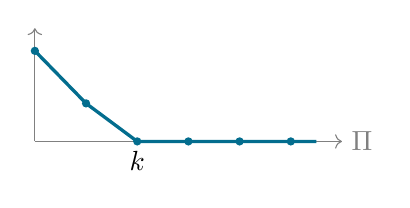
\begin{tikzpicture}[x=.65cm,y=1.15cm]
\draw[->,gray] (0,0)--(6.0,0) node[right] {$ \Pi $};
\draw[->,gray] (0,0)--(0,1.25);
\draw[tealBlue,very thick] (0,1)--(1,.42)--(2,0)--(5.5,0);
\foreach \x/\y in {0/1,1/.42,2/0,3/0,4/0,5/0}{\fill[tealBlue] (\x,\y) circle (1.5pt);}
\node[below] at (2,0) {$k$};
\end{tikzpicture}
\par\smallskip\centerline{$P^k=\Pi$}
\column{.48\textwidth}
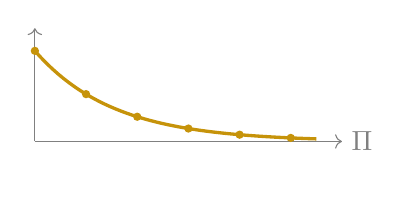
\begin{tikzpicture}[x=.65cm,y=1.15cm]
\draw[->,gray] (0,0)--(6.0,0) node[right] {$\Pi$};
\draw[->,gray] (0,0)--(0,1.25);
\draw[CPPGold,very thick] plot[domain=0:5.5,samples=50] (\x,{exp(-.65*\x)});
\foreach \x in {0,...,5}{\fill[CPPGold] (\x,{exp(-.65*\x)}) circle (1.5pt);}
\node[below,opacity=0] at (2,0) {$k$};
\end{tikzpicture}
\par\smallskip\centerline{$P^m\longrightarrow\Pi$}
\end{columns}
\end{frame}

\begin{frame}{A 4 state example}


\begin{center}
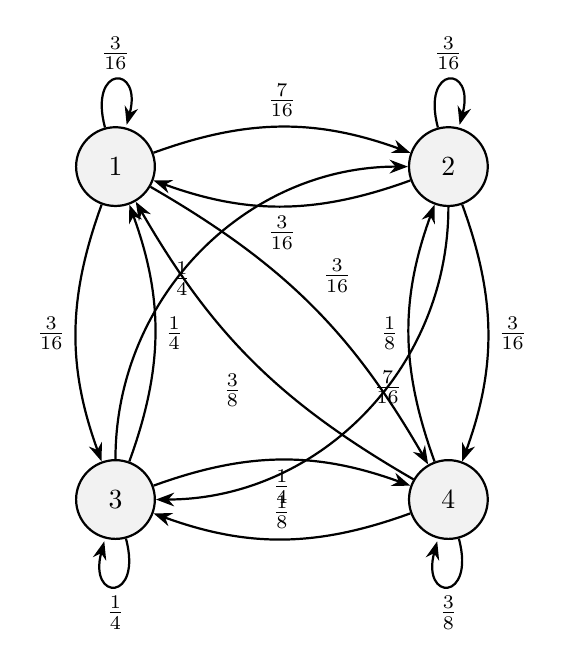
\begin{tikzpicture}[
    ->, 
    >=Stealth, 
    node distance=3.2cm, 
    every state/.style={thick, fill=gray!10, minimum size=1cm}, 
    thick
]

  % States arranged in a square layout
  \node[state] (1) {$1$};
  \node[state, right=of 1] (2) {$2$};
  \node[state, below=of 2] (4) {$4$};
  \node[state, left=of 4] (3) {$3$};

  % Transitions from State 1
  \draw (1) edge[loop above] node[above] {$\frac{3}{16}$} (1);
  \draw (1) edge[bend left=20] node[above] {$\frac{7}{16}$} (2);
  \draw (1) edge[bend right=20] node[left] {$\frac{3}{16}$} (3);
  \draw (1) edge[bend left=15] node[above right=1pt] {$\frac{3}{16}$} (4);

  % Transitions from State 2
  \draw (2) edge[bend left=20] node[below] {$\frac{3}{16}$} (1);
  \draw (2) edge[loop above] node[above] {$\frac{3}{16}$} (2);
  \draw (2) edge[bend left=20] node[right] {$\frac{3}{16}$} (4);
  \draw (2) edge[bend left=45] node[above right] {$\frac{7}{16}$} (3);

  % Transitions from State 3
  \draw (3) edge[bend right=20] node[right] {$\frac{1}{4}$} (1);
  \draw (3) edge[bend left=45] node[below left] {$\frac{1}{4}$} (2);
  \draw (3) edge[loop below] node[below] {$\frac{1}{4}$} (3);
  \draw (3) edge[bend left=20] node[below] {$\frac{1}{4}$} (4);

  % Transitions from State 4
  \draw (4) edge[bend left=15] node[below left=1pt] {$\frac{3}{8}$} (1);
  \draw (4) edge[bend left=20] node[left] {$\frac{1}{8}$} (2);
  \draw (4) edge[bend left=20] node[above] {$\frac{1}{8}$} (3);
  \draw (4) edge[loop below] node[below] {$\frac{3}{8}$} (4);

\end{tikzpicture}
\end{center}
\end{frame}

\begin{frame}{A 4 State Example}
\begin{columns}[c]

  % Left column: P and P^2
  \begin{column}{0.48\textwidth}
    \small
    \[
    P = \begin{pmatrix}
    \frac{3}{16} & \frac{7}{16} & \frac{3}{16} & \frac{3}{16} \\[3pt]
    \frac{3}{16} & \frac{3}{16} & \frac{7}{16} & \frac{3}{16} \\[3pt]
    \frac{1}{4}  & \frac{1}{4}  & \frac{1}{4}  & \frac{1}{4}  \\[3pt]
    \frac{3}{8}  & \frac{1}{8}  & \frac{1}{8}  & \frac{3}{8}
    \end{pmatrix}
    \]

    \[
    P^2 = \begin{pmatrix}
    \frac{15}{64} & \frac{15}{64} & \frac{19}{64} & \frac{15}{64} \\[3pt]
    \frac{1}{4}   & \frac{1}{4}   & \frac{1}{4}   & \frac{1}{4}   \\[3pt]
    \frac{1}{4}   & \frac{1}{4}   & \frac{1}{4}   & \frac{1}{4}   \\[3pt]
    \frac{17}{64} & \frac{17}{64} & \frac{13}{64} & \frac{17}{64}
    \end{pmatrix}
    \]

  \end{column}

  % Right column: P^3
  \begin{column}{0.48\textwidth}
    \small
    \[
    P^3 = \begin{pmatrix}
    \frac{1}{4} & \frac{1}{4} & \frac{1}{4} & \frac{1}{4} \\[3pt]
    \frac{1}{4} & \frac{1}{4} & \frac{1}{4} & \frac{1}{4} \\[3pt]
    \frac{1}{4} & \frac{1}{4} & \frac{1}{4} & \frac{1}{4} \\[3pt]
    \frac{1}{4} & \frac{1}{4} & \frac{1}{4} & \frac{1}{4}
    \end{pmatrix} = \Pi
    \]
    \[
    \pi = \frac{1}{4},\frac{1}{4},\frac{1}{4},\frac{1}{4}
    \]
  \end{column}

\end{columns}
\end{frame}
\begin{frame}{An n-1 steady state generator}
\textbf{Construction:} For $r \ge 3$, define $P_r$ by
\begin{equation}
(P_n)_{ij} = \begin{cases}
\dfrac{2n - 1}{n^2}, & 1 \le i \le n - 2, \ j = i + 1, \\[8pt]
\dfrac{n - 1}{n^2}, & 1 \le i \le n - 2, \ j \neq i + 1, \\[8pt]
\dfrac{1}{n}, & i = n- 1, \\[8pt]
\dfrac{2(n - 1)}{n^2}, & i = n, \ j \in \{1, n\}, \\[8pt]
\dfrac{n - 2}{n^2}, & i = n, \ 2 \le j \le n - 1.
\end{cases}
\end{equation}
Here
\[
P_n^{n-2} \neq J_n, \qquad P_n^{n-1} = J_n.
\]


Every entry of $P_n$ is strictly positive. The matrix is doubly stochastic, so its invariant distribution is uniform. Positivity makes the chain irreducible and aperiodic. Hence the first steady-state power is exactly $P_r^{n-1}$.

\end{frame}
%\begin{frame}    
%\begin{itemize}
%    \item<1-> Text visible on slide 1
%    \item<2-> Text visible on slide 2
%    \item<3> Text visible on slides 3
%    \item<4-> Text visible on slide 4
%\end{itemize}
%\end{frame}

\begin{frame}{}
    \begin{block}{Conjecture}
A markov chain that reaches its steady state has one eigenvalue of 1, with the rest being zero.  

\end{block}

 \begin{block}{Distinct eigenvalues: Sylvester's expansion}
With $\lambda_1=1$, $A_1=\Pi$, and
$|\lambda_i|<1$ for $i\ge2$,
\[
P^m=\sum_{i=1}^{n}\lambda_i^m A_i
   =\Pi+\sum_{i=2}^{n}\lambda_i^m A_i.
\]
Here $A_i$ is the spectral projector for $\lambda_i$.
\end{block}

\end{frame}


    
%-----\begin{frame}{Example: $\lambda_1=1, \lambda_2=\frac{1}{2}$}\lambda 1=1
\begin{frame}{Example $\lambda_1=1, \lambda_i =\frac{1}{2} $}
\[
P_{1/2}=\begin{pmatrix}5/6&1/6\\1/3&2/3\end{pmatrix},
\qquad \mu_0=(1,0).
\]
\[
\Pr(X_m=0)=\frac23+\frac13\left(\frac12\right)^m.
\]
\begin{center}
\begin{tikzpicture}
\begin{axis}[talkaxis]
\addplot[gray,dashed,domain=0:8.1] {2/3};
\addplot[tealBlue,very thick,mark=*,samples at={0,1,2,3,4,5,6,7,8}] {2/3+1/3*(.5)^x};
\node[anchor=south east,font=\small,text=tealBlue] at (axis cs:7.7,.80) {$\pivec=(2/3,1/3)$};
\end{axis}
\end{tikzpicture}
\end{center}
\end{frame}

\begin{frame}{Example: $\lambda_1=1, \lambda_i=0$}
\[
P = \begin{pmatrix} 1/2 & 1/2 \\ 1/2 & 1/2 \end{pmatrix},
\qquad \mu_0=(1,0).
\]
\[
\Pr(X_m=0) = \frac{1}{2} + \frac{1}{2}\delta_{m,0}.
\]
\begin{center}
\begin{tikzpicture}
\begin{axis}[talkaxis, ymin=0, ymax=1.1]
\addplot[gray,dashed,domain=0:8.1] {0.5};
\addplot[tealBlue,very thick,mark=*,samples at={0,1,2,3,4,5,6,7,8}] { (x==0) ? 1 : 0.5 };
\node[anchor=south east,font=\small,text=tealBlue] at (axis cs:7.7,0.7) {$\pivec=(1/2,1/2)$};
\end{axis}
\end{tikzpicture}
\end{center}
\end{frame}

\begin{frame}{An attempt at a Generalization}


Let P be some markov chain with a with a finite step steady state,  $m \in \mathbb{N}$
\[
 P^m = \Pi + N^m
\]
where at some finite-step k
\[
 P^k = \Pi
\]

Since the chain reaches its steady state at some finite step $k$, $P^k = \Pi$, which implies $N^k = 0$. Thus, $N$ is a nilpotent matrix.

%By Jordan Canonical Form properties, the maximum index of nilpotency on an $(n-1)$-dimensional vector space is $n-1$.

%Therefore, absolute finite-step convergence can only occur when $k \le n-1$. 

%Which means that any Finite-Step Markov Chain will hit its steady state in less steps than its size. 
\medskip
By Jordan Canonical Form, the maximum nilpotent block size in an $(n-1)$-dimensional subspace is $(n-1) \times (n-1)$.

\vskip 1em % Forces the space before the line
\hrule
\vskip 1em % Forces the space after the line

Therefore, absolute finite-step convergence can only occur when $k \le n-1$.


\end{frame}    
\begin{frame}{References}
\footnotesize
\begin{thebibliography}{9}
%why emoji?? I can't figure how to remove without removing \bibterm.

\bibitem{rumble2026}
        Douglas W. Rumble.
        \newblock \emph{Jordan Form and Nilpotent Matrices}.
        \newblock Millersville University Department of Mathematics.
        \newblock Available online: \url{https://sites.millersville.edu/rumble/Math.422/jordannil.pdf}

\bibitem{hoel1972}
Hoel, P. G., Port, S. C., \& Stone, C. J. (1972).
\newblock \emph{Introduction to Stochastic Processes}.
\newblock Chapter 4.1: Mean and Covariance Functions, pp. 110--119.

\bibitem{meyer2023}
Meyer, C. D. (2023).
\newblock \emph{Matrix Analysis and Applied Linear Algebra}.
\newblock Society for Industrial and Applied Mathematics.

\bibitem{parzen1967}
Parzen, E. (1967).
\newblock \emph{Stochastic Processes}.
\newblock Random Variables and Stochastic Processes, pp. 7--40.
\newblock \url{https://doi.org/10.1137/1.9781611971120.ch1.ch6}


\end{thebibliography}
\end{frame}


%---------------------------------------------------------




\end{document}
